Nesta seção, será explicado como pretende-se desenvolver o módulo de teste de performance que vai ser acoplado no my5G-RAN Tester\footnote{\url{https://github.com/my5G/my5G-RANTester}}.
Com o intuito de avaliar o comportamento das diferentes implementações \textit{open source} de núcleo 5G para execução dos procedimentos em escala e utilizando-se como base a prova de conceito do trabalho de \cite{Dominato2021}, propõe-se desenvolver uma extensão para a aplicação my5G-RANTester.
Uma arquitetura em alto nível da aplicação a ser desenvolvida pode ser vista na Figura \ref{fig:tester_arch}.

\begin{figure}[!ht]
    \centering
    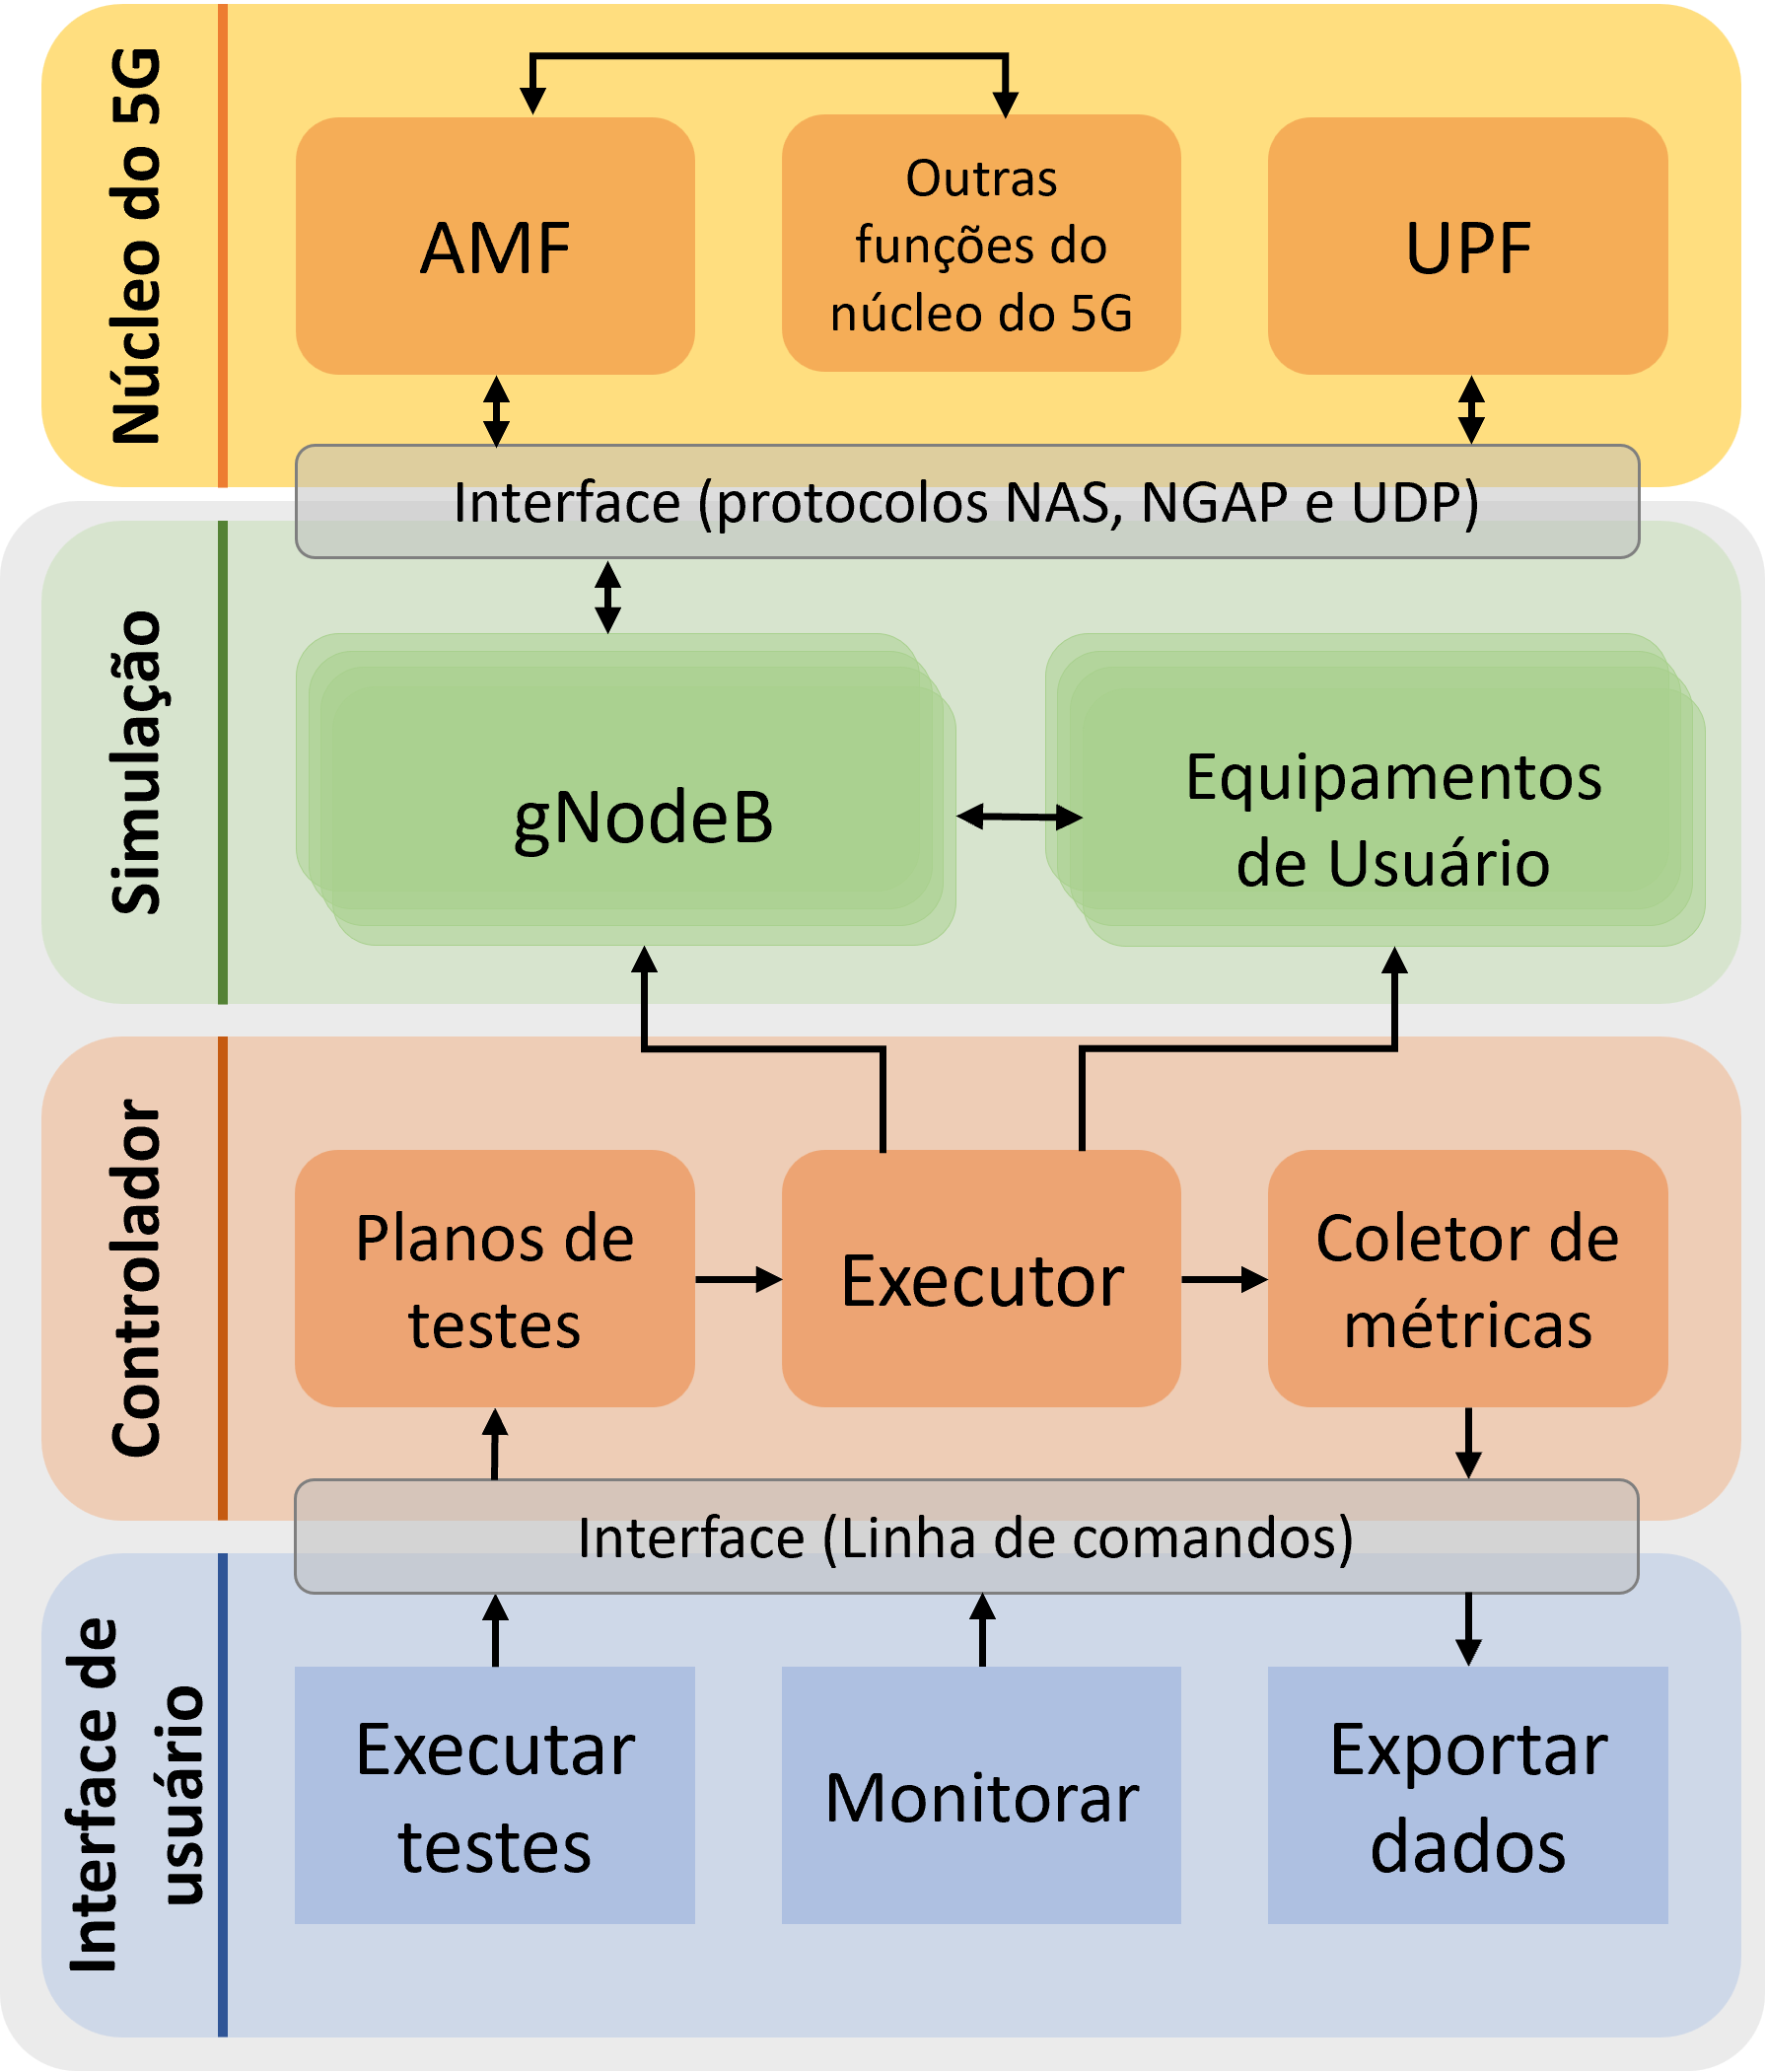
\includegraphics[width=0.6\textwidth]{TG1/Images/TesterArchtectureV2.png}
    \caption{Arquitetura do trabalho}
    \label{fig:tester_arch}
\end{figure}

A camada superior da Figura \ref{fig:tester_arch} representa o núcleo da rede a ser testado. O núcleo em teste implementa uma interface de comunicação que aceita chamadas para a função AMF utilizando-se os protocolos NAS e NGAP. Essa interface também utiliza o protocolo UDP para a comunicação com a função UPF, responsável pelo plano de usuário.

A prova de conceito implementa as três camadas inferiores, sendo elas as camadas de Simulação, do Controlador e da Interface de usuário.
A camada de Simulação irá simular o comportamento de uma ou mais gNodeB e de um ou mais equipamentos de usuário.
Nessa camada, a diferença entre a implementação feita no trabalho de \cite{Dominato2021} e o que será feito no presente trabalho é a capacidade de simular múltiplas gNodeB e UEs simultaneamente, com o intuito de validar a performance de cada implementação de núcleo da rede.

A camada do Controlador é a principal camada no funcionamento do testador. Essa camada recebe os comandos do usuário através de uma interface que define qual teste será executado, controla a camada acima e faz a coleta e o armazenamento das métricas do experimento.
Os planos de testes representam os testes em si que serão escolhidos para serem executados. O Executor recebe as informações do teste e configura as gNodeB e os UEs e envia as métricas para o Coletor de métricas, que irá armazená-las para futuros usos.

Por fim, a camada da Interface de usuário permitirá a execução e o monitoramento dos testes, além de exportar as métricas armazenadas na camada acima. É com essa camada que o usuário do testador irá interagir através de parâmetros enviados por uma linha de comandos a ser executada no ambiente de testes.

A implementação a ser usada como base é feita na linguagem \textit{Go}, criada pela Google em 2009\footnote{https://go.dev/}. O objetivo desse trabalho é estender o testador existente, adicionando a funcionalidade de testes de desempenho.
Para analisar o desempenho das implementações \textit{open source} de núcleos 5G, as métricas a serem coletadas são latência, perda de pacotes da rede e uso de processador e memória RAM da máquina usada para realizar os testes.

\begin{table}[!ht]
\centering
\caption{Configuração da máquina de testes}
\label{tab:vm-config}
\begin{tabular}{lr}
\hline
 & \multicolumn{1}{c}{\textbf{Máquina Virtual}} \\ \hline
\textbf{CPU} & \begin{tabular}[c]{@{}r@{}}Intel Core i9 12900\\ @ 2.4 GHz e 16 núcleos\end{tabular} \\ \hline
\textbf{Memória RAM} & 32 GB DDR5-4800 \\ \hline
\textbf{Armazenamento} & SSD M.2 128 GB NVMe \\ \hline
\end{tabular}
\end{table}

Pretende-se aplicar os testes de desempenho sobre os núcleos \textit{free5GC}, \textit{Open5GS} e \textit{OpenAirInterface}. Os testes serão executados em uma máquina virtual rodando o sistema operacional Ubuntu 20.04 LTS com as seguintes configurações de hardware: processador Intel Core i9 12900, contendo 16 núcleos e 32 GB de memória RAM dedicados, além de 128 GB de armazenamento em um SSD M.2 NVMe. Ao utilizar-se equipamentos de alto desempenho, pretende-se extrair o máximo desempenho dos núcleos de rede 5G, permitindo a conexão de múltiplos equipamentos de usuários e gNodeB e avaliando o comportamento desses núcleos nessa situação. A Tabela \ref{tab:vm-config} exibe o hardware a ser utilizado nos testes.
